% !TEX encoding = UTF-8 Unicode
\documentclass[a4paper]{article}

\usepackage{color}
\usepackage{url}
\usepackage[T2A]{fontenc} % enable Cyrillic fonts
\usepackage[utf8]{inputenc} % make weird characters work
\usepackage{graphicx}

%\usepackage[english,serbian]{babel}
\usepackage[english,serbianc]{babel} %ukljuciti babel sa ovim opcijama, umesto gornjim, ukoliko se koristi cirilica

\usepackage[unicode]{hyperref}
\hypersetup{colorlinks,citecolor=green,filecolor=green,linkcolor=blue,urlcolor=blue}

\usepackage{listings}
\usepackage{amsmath}

\newtheorem{primer}{Пример}[section] %ćirilični primer
% \newtheorem{primer}{Primer}[section]

\definecolor{mygreen}{rgb}{0,0.6,0}
\definecolor{mygray}{rgb}{0.5,0.5,0.5}
\definecolor{mymauve}{rgb}{0.58,0,0.82}

\lstset{ 
  backgroundcolor=\color{white},   % choose the background color; you must add \usepackage{color} or \usepackage{xcolor}; should come as last argument
  basicstyle=\scriptsize\ttfamily,        % the size of the fonts that are used for the code
  breakatwhitespace=false,         % sets if automatic breaks should only happen at whitespace
  breaklines=true,                 % sets automatic line breaking
  captionpos=b,                    % sets the caption-position to bottom
  commentstyle=\color{mygreen},    % comment style
  deletekeywords={...},            % if you want to delete keywords from the given language
  escapeinside={\%*}{*)},          % if you want to add LaTeX within your code
  extendedchars=true,              % lets you use non-ASCII characters; for 8-bits encodings only, does not work with UTF-8
  firstnumber=1000,                % start line enumeration with line 1000
  frame=single,	                   % adds a frame around the code
  keepspaces=true,                 % keeps spaces in text, useful for keeping indentation of code (possibly needs columns=flexible)
  keywordstyle=\color{blue},       % keyword style
  language=Python,                 % the language of the code
  morekeywords={*,...},            % if you want to add more keywords to the set
  numbers=left,                    % where to put the line-numbers; possible values are (none, left, right)
  numbersep=5pt,                   % how far the line-numbers are from the code
  numberstyle=\tiny\color{mygray}, % the style that is used for the line-numbers
  rulecolor=\color{black},         % if not set, the frame-color may be changed on line-breaks within not-black text (e.g. comments (green here))
  showspaces=false,                % show spaces everywhere adding particular underscores; it overrides 'showstringspaces'
  showstringspaces=false,          % underline spaces within strings only
  showtabs=false,                  % show tabs within strings adding particular underscores
  stepnumber=2,                    % the step between two line-numbers. If it's 1, each line will be numbered
  stringstyle=\color{mymauve},     % string literal style
  tabsize=2,	                   % sets default tabsize to 2 spaces
  title=\lstname                   % show the filename of files included with \lstinputlisting; also try caption instead of title
}

\begin{document}

\title{Генетичко програмирање\\ \small{Семинарски рад у оквиру курса\\Методологија стручног и научног рада\\ Математички факултет}}

\author{Александра Стојановић, Ивана Ивановић,\\ Александар Стефановић, Оливера Поповић\\ mi16048@alas.matf.bg.ac.rs, mi16120@alas.matf.bg.ac.rs,\\ ai16222@alas.matf.bg.ac.rs, mi16064@alas.matf.bg.ac.rs}

%\date{9.~april 2015.}

\maketitle

\abstract{
U ovom tekstu je ukratko prikazana osnovna forma seminarskog rada. Obratite pažnju da je pored ove .pdf datoteke, u prilogu i odgovarajuća .tex datoteka, kao i .bib datoteka korišćena za generisanje literature. Na prvoj strani seminarskog rada su naslov, apstrakt i sadržaj, i to sve mora da stane na prvu stranu! Kako bi Vaš seminarski zadovoljio standarde i očekivanja, koristite uputstva i materijale sa predavanja na temu pisanja seminarskih radova. Ovo je samo šablon koji se odnosi na fizički izgled seminarskog rada (šablon koji \emph{morate} da koristite!) kao i par tehničkih pomoćnih uputstava. Pročitajte tekst pažljivo jer on sadrži i važne informacije vezane za zahteve obima i karakteristika seminarskog rada.}

\tableofcontents

\newpage

\section{Увод}
\label{sec:uvod}



Kada budete predavali seminarski rad, imenujete datoteke tako da sadrže redni broj teme, temu seminarskog rada, kao i prezimena članova grupe. Precizna uputstva na temu imenovnja će biti data na formi za predaju seminarskog rada. Predaja seminarskih radova biće isključivo preko veb forme, a NE slanjem mejla. Link na formu će biti dat u okviru obaveštenja na strani kursa. Vodite računa da prilikom predavanja seminarskog rada predate samo one fajlove koji su neophodni za ponovno generisanje pdf datoteke. To znači da pomoćne fajlove, kao što su .log, .out, .blg, .toc, .aux i slično, \textbf{ne treba predavati}.

\section{Историјат}

\section{Опис методе}

Генетичко програмирање је метода која је настала као један од покушаја да се спроведе аутоматизација прављења рачунарских програма за решавања проблема задатих на веома апстрактном нивоу. Основни циљ је да ови проблеми буду тако дефинисани да је познато једино шта треба да буде урађено, без додатних информација о форми или структури решења.\newline

Идеја на којој ова метода почива је процес еволуције који се јавља у природи. Самим тим, генетичко програмирање је техника која спада у групу алгоритама  \textbf{еволутивног израчунавања} \cite{compIntelligence}. Еволуција подразумева промену особина укупне популације кроз више смењених генерација. Постојало је током времена више теорија еволуције, док је данас опште прихваћена теорија чији је творац британски биолог Чарлс Роберт Дарвин. По његовој теорији, сви живи организми се развијају процесом природне селекције \cite{darwin1859}. Тим процесом јединке које су боље прилагођене имају већу вероватноћу да преживе и да оставе потомство, које је углавном једнако или чак и боље прилагођено од родитеља. Да би могли да оставе потомство, у ћелијама сваког живог бића постоје хромозоми, који су сачињени од гена. Ген је основна јединица наслеђивања, која преноси поруке из генерације у генерацију. Дакле, репродукција подразумева комбинацију гена родитеља уз мале количине мутације. Карактеристике, односно генетски материјал прилагођених јединки углавном опстаје кроз генерације и у неком тренутку почиње да доминира, док остале особине најчешће ишчезну.\newline
%  На тај начин јединке преносе своје карактеристике на наредне генерације, али се истовремено добијају и нове.

У овом одељку биће описано како се процес еволуције осликава на генетичко програмирање, које су његове основне компоненте као и то које одлуке треба донети при прилагођавању алгоритма задатом проблему.

\subsection{Општи алгоритам}

У генетичком програмирању популацију чине рачунарски програми. Еволуцијом се од почетних, најчешће на случајан начин генерисаних програма, добијају нови, у нади бољи и ефикаснији програми. Обзиром да је то случајан процес, резултат никада не може бити гарантован. Ипак, управо та случајност даје могућност превазилажења неких проблема које имају други детерминистички алгоритми \cite{fieldGuidetoGP}. 

На слици \ref{fig:kontrola_toka} приказан је дијаграм контроле тока опште верзије алгоритма. У наредним поглављима биће детаљно описан сваки од наведених корака алгоритма.

\begin{figure}[h!]
    \begin{center}
        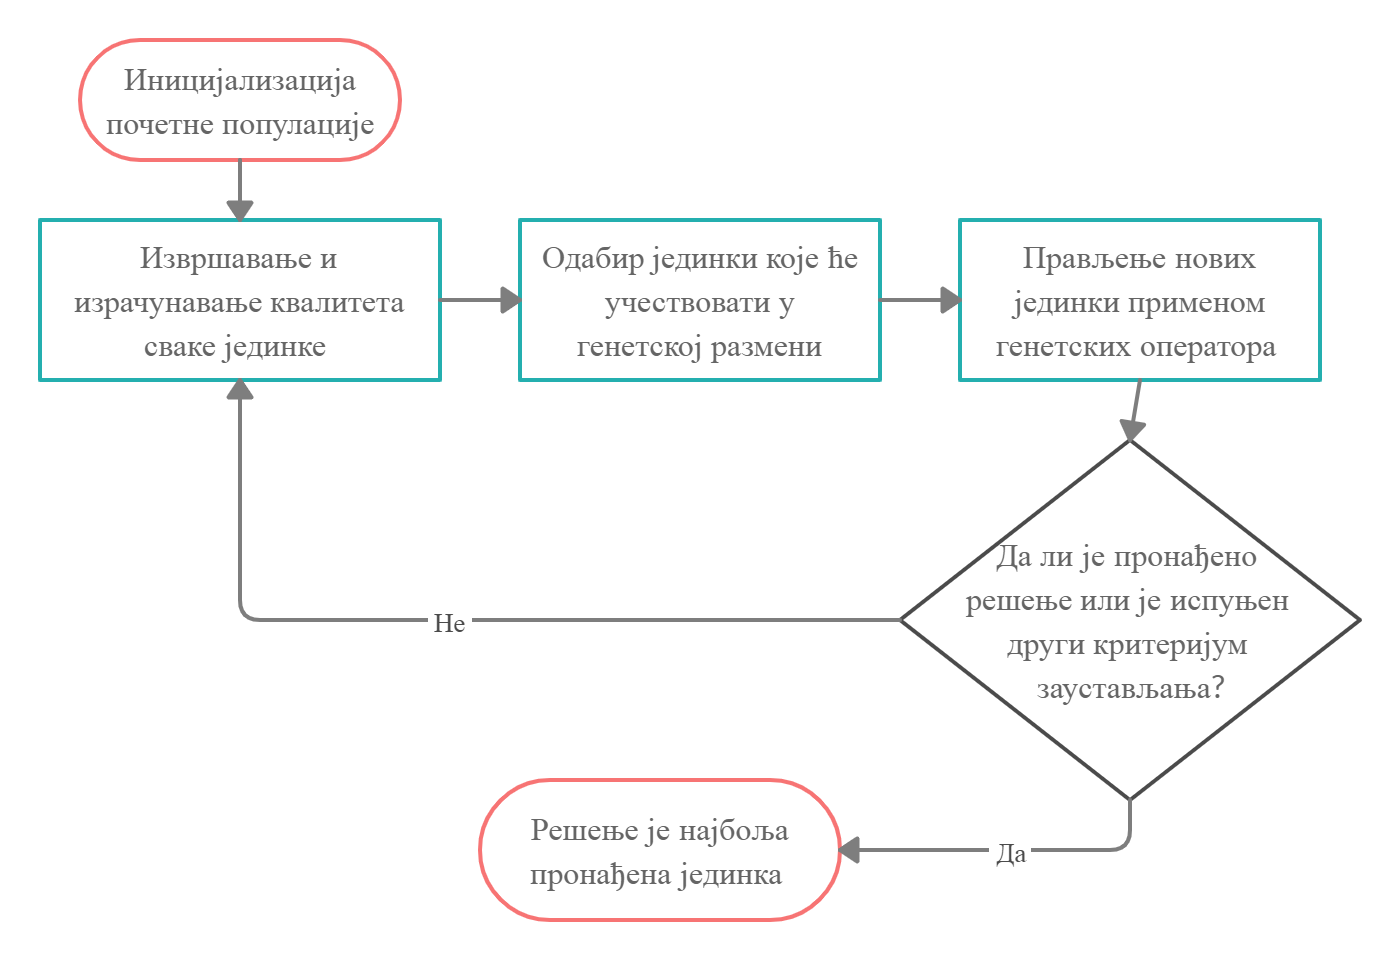
\includegraphics[scale=0.22]{opstiAlgoritam.png}
    \end{center}
    \caption{Општи алгоритам генетичког програмирања}
    \label{fig:kontrola_toka}
\end{figure}

\subsubsection{Репрезентација јединки}

У генетичком програмирању, јединке су заправо рачунарски програми који се могу извршавати. Ипак, иако то на први поглед делује логично, оне неће бити представљене линијама кода. Разлог томе је што је неопходно да над изабраном репрезентацијом буду дефинисани генетски оператори (више о њима у наредним секцијама \ref{sec:reprodukcija} и \ref{sec:mutacija}), а да извршавање буде ефикасно. Репрезентација која то испуњава је она у виду \textbf{синтаксних стабала} \cite{synTrees}, те се она најчешће користи.\newline

Код синтаксних стабала, основно је да се променљиве и константе налазе у листовима (најнижи чворови) и називају се терминалима, док се у осталим чворовима налазе функције. Функције могу бити различите природе, на пример аритметичке, тригонометријске или логичке, али могу бити и различите програмске конструкције попут условних израза и петљи. Свако овакво стабло мора имати скуп дефинисаних терминала и функција који заједно чине такозвани \textbf{примитивни скуп} генетичког програмирања. 

\begin{primer}
    Нека је проблем задат аритметичком формулом: 
    \begin{equation} 
        \label{eq:sintaksno_stablo}
        2*\pi-\frac{5+x}{y-4}
    \end{equation}
    Одговарајући скуп терминала: \{2, $\pi$, 5, x, y, 4\}, скуп функција:\newline \{+, -, *, /\}, док је одговарајуће синтаксно стабло дато на слици \ref{fig:sintaksno_stablo}.

    \begin{figure}[h!]
        \begin{center}
        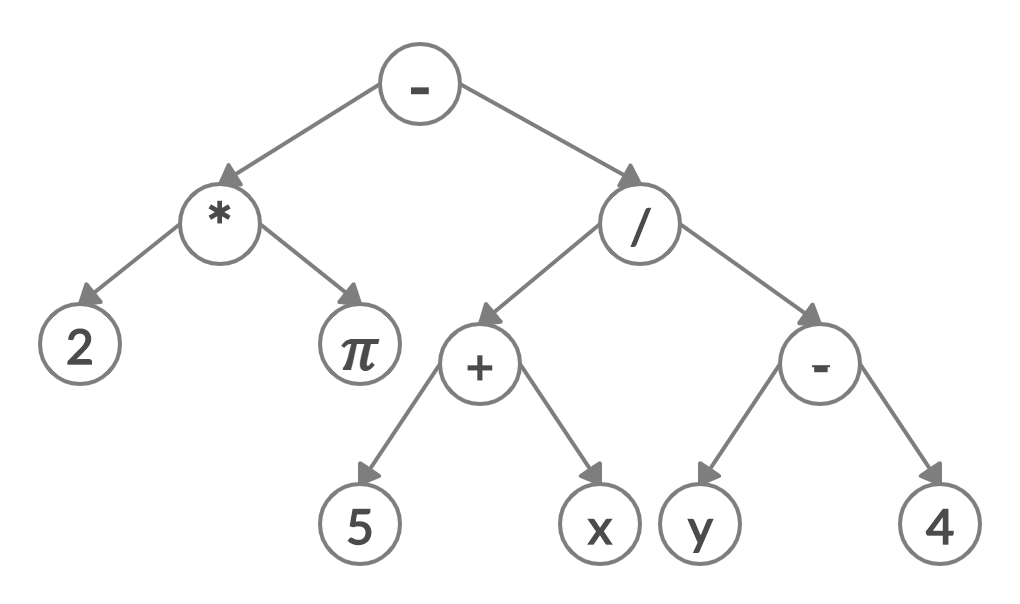
\includegraphics[scale=0.22]{sintaksnoStablo.png}
        \end{center}
        \caption{Синтаксно стабло које одговара формули \eqref{eq:sintaksno_stablo}}
        \label{fig:sintaksno_stablo}
    \end{figure}
\end{primer}


Репрезентација стаблима има неколико импликација које треба имати на уму \cite{compIntelligence}:
\begin{itemize}
    \item Величина (висина), облик (какве су гране чворова) и сложеност јединки нису фиксирани, већ се могу разликовати. Те особине се чак и код једне јединке такође могу мењати током времена, услед примене оператора за репродукцију.
    \item За сваки проблем се посебно мора дефинисати граматика, односно мора се дефинисати примитиван скуп тако да је њиме могуће представити сва могућа решења. Као додатак примитивном скупу, могу бити дефинисана и семантичка правила која обезбеђују конструкцију исправних стабала. На пример, једно такво правило могло би да буде да делилац никада не сме да буде једнак 0.
\end{itemize}

Некада се може испоставити да је репрезентација стаблима недовољно удобна за рад јер захтева управљање великим бројем показивача. Најчешће велика већина функција које се користе има фиксирану арност (број аргумената), што омогућава да се стабла прикажу као линеарне структуре (листе, низови). Која ће се репрезентација користити зависи највише од домена проблема који се решава \cite{fieldGuidetoGP}.

\subsubsection{Иницијализација популације}

Генерисање почетне популације обично се врши на случајан начин, при чему се поштују сва дефинисана ограничења, уколико она постоје. Две најстарије и најједноставније методе су \textbf{потпуна метода} (eng.~{\em full method}) и \textbf{метода раста} (eng.~{\em grow method}), као и њихова широко распрострањена пола-пола комбинација \cite{fieldGuidetoGP}. Да би се разумеле ове две методе, потребно је прво увести две дефиниције:

\begin{itemize}
    \item \textbf{Дубина чвора} представља број грана које треба прећи да би се од корена дошло до тог чвора. Корен се подразумевано налази на дубини 0.\newline
    \emph{Дубина чвора са вредношћу $\pi$ приказаног на слици \ref{fig:sintaksno_stablo} износи \underline{2}.}
    \item \textbf{Дубина читавог стабла} је дубина његовог најдубљег листа.
    \emph{Дубина стабла приказаног на слици \ref{fig:sintaksno_stablo} износи \underline{3}.}
\end{itemize}

Прва метода зове се потпуна јер креира потпуна стабла. Стабло је потпуно уколико су му сви листови на истој дубини. По овој методи, чворови се бирају на случајан начин све док се не дође до максималне дубине. Након тога се бирају на случајан начин из скупа терминала. По другој методи, методи раста, чворови се бирају на случајан начин из целог примитивног скупа док се не дође до максималне дубине, а након тога се исто бирају само терминали. Основна разлика између ове две методе је што метода раста дозвољава креацију стабала са више различитих величина и облика.\newline

Ипак, ниједна од ове две методе не пружа претерано велику разноврсност. Због тога се данас нашироко користи њихова комбинација коју је предложио Џон Коза. Она подразумева да се половина генерације креира коришћењем потпуне методе, а друга половина методом раста.

\subsubsection{Функција прилагођености}

Функција прилагођености (eng.~{\em fitness function}) даје оцену \textbf{квалитета јединке}. Она треба да буде одабрана тако да може да се израчуна за сваку јединку а да израчунавање притом буде што ефикасније \cite{vi}. Зависи од проблема који се решава, али се у генетичком програмирању најчешће реализује тако што постоји скуп тест случајева којима се свака јединка евалуира. То значи да постоји одређени број улаза за које се знају очекивани излази, па се евалуира колико излаза је јединка, односно програм погодио.
Осим као мера квалитета јединке, функција прилагођености се такође може користити да додели пенале оним јединкама које нису прихватљиве или нису семантички тачне.

\subsubsection{Селекција}

Селекција се користи како би се пронашле боље прилагођене јединке које ће учествовати у репродукцији. То се врши коришћењем функције прилагођености. На основу њене вредности јединке се узимају са одређеном вероватноћом. Најчешће се користе \textbf{турнирска селекција} и селекција пропорционала вредности функције прилагођености, али се могу користити и друге селекционе методе еволутивног израчунавања. Код турнирске селекције бира се одређени број јединки из популације, на случајан начин. Оне се упоређују и бира се најбоља од њих, која ће учествовати у репродукцији. Постоје и разне друге варијанте турнирске селекције, али је њена предност свакако то што и средње квалитетне јединке могу добити шансу да оставе потомке. Пример селекције пропроционалне вредности функције прилагођености је \textbf{рулетска селекција} (eng.~{\em roulette wheel selection}). По њој, вероватноћа да ће јединка бити изабрана једнака је: 
\begin{equation} 
    p_i = \frac{f(i)}{\sum_{j}^{N} f(i)}
\end{equation}
где је f(i) вредност функције прилагођености јединке i, док је N укупан број јединки у популацији \cite{vi}.

\subsubsection{Репродукција}
\label{sec:reprodukcija}

Репродукција представља начин на који се од два селекцијом изабрана родитеља добиј потомство. Код генетичког програмиранја најчешће се користи метод укрштања подстабала. На случајан начин одаберу се тачке укрштања код оба родитеља, након чега се једноставно замене подстабла родитеља са кореном у тачки укрштања. Постоје две опције, креирање једног или два детета разменом. Проблем код овог метода је то што се најчешће барата са стаблима код којих сваки чвор има најмање двоје деце, што доводи до тога да већи број чворова припада скупу терминала. Последица тога је што се размењују мање количине генетског материјала, јер се чешће на случајан начин погоди управо неки од терминала. Да би се избегао овај проблем, Коза је 1992. предложио нашироко коришћен приступ бирања функција 90\% времена, а листова преосталих 10\%. Постоји још много видова репродукције који се користе код генетичког програмирања \cite{fieldGuidetoGP}.

\subsubsection{Мутација}
\label{sec:mutacija}

Мутација се примењује како током времена јединке не би постале сувише сличне. Такође помаже у избегавању локалних екстремума, у ком би се највероватније јединке заглавиле уколико не би било мутације.
Мутација се најчешће имплементира тако да се на случајан начин изабере тачка јединке, па се подстабло са кореном у тој тачки замени случајно генерисаним стаблом. Још један чест начин имплементације је да се такође на случајан начин изабере тачка у стаблу јединке, али се сада вредност у том чвору замени случајно одабраним

\section{Примери примене}
Примена генетичког програмирања у индустрији је разнолико и рапидно се повећава годинама. Споменућемо неке од важнијих радова написаних о изабраним темама.
\subsection{Гејминг}
\subsection{Роботика}
Један од проблема у роботици укључује два агента А и Б који управљају својим возилима на дводимензионалној мрежи. Возила се све време померају у правцу у коме је возило окренуто. Сви покрети су дискретни, тако да возила имају увек целобројне (x, y) координате. Иницијално возила су окренута ка северу, а механизам управљања возилом дозвољава окретање возила у једном од 8 географских праваца. Циљ је да агенти А и Б својим возилима дођу један до другог.

Агенти А и Б имају информацију само о сопственој позицији, али такође имају приступ каналима за комуникацију КаналА и КаналБ који се могу користити за слање и примање порука од другог агента. Сваки комуникациони канал је конектован са једним возилом, тако да порука послата са једног краја може бити примљена само на другом крају и обрнуто. \cite{robo0}

Сличан овоме, проблем пре тога укључивао је два играча у возилима који су се играли јурке. С тим што је овде сваки играч имао информацију о томе ко јури и где му се апроксимативно налази противник. Циљ је што краће бити онај који треба да јури противника. Играју се четири игре, смењујући се у свакој рунди ко први јури. У току једне рунде улоге се мењају кад онај који јури буде од свог противника на дужини од једног возила. Свака рунда се састоји из 25 симулација, где је играчев резултат за ту рунду рачунат као број колико пута није био онај који јури подељен са 25. \cite{robo1}

Такође, постоји и проблем навигације робота како би нашао храну која је постављена дуж неправилне линије; где робот зна да извршава примитивне операције: померање напред, окретање лево/десно као и мирисање хране. Путање које су коришћене су:
\begin{itemize}
	\item "Santa Fe" путања (приказана на слици \ref{fig:santa_fe}) - направљена од 89 комада хране, где између њих постоји једна, две или три празнине без хране који могу бити и на угловима линије кретања робота
	\item "Los Altos Hills" путања - састављена од 157 комада хране, где 105. комад представља 89. комад из претходне путање. Након тог комада, додате су још две ирегуларности у путањи:
	\begin{itemize}
		\item[$-$] налажење хране два места лево или десно од претходног комада хране; прво појављивање после 116. комада хране 
		\item[$-$] померање једно место унапред, а онда проналажење хране два месте лево или десно; прво појављивање после 136. комада хране
	\end{itemize}
\end{itemize}

\begin{figure}[h!]
    \begin{center}
        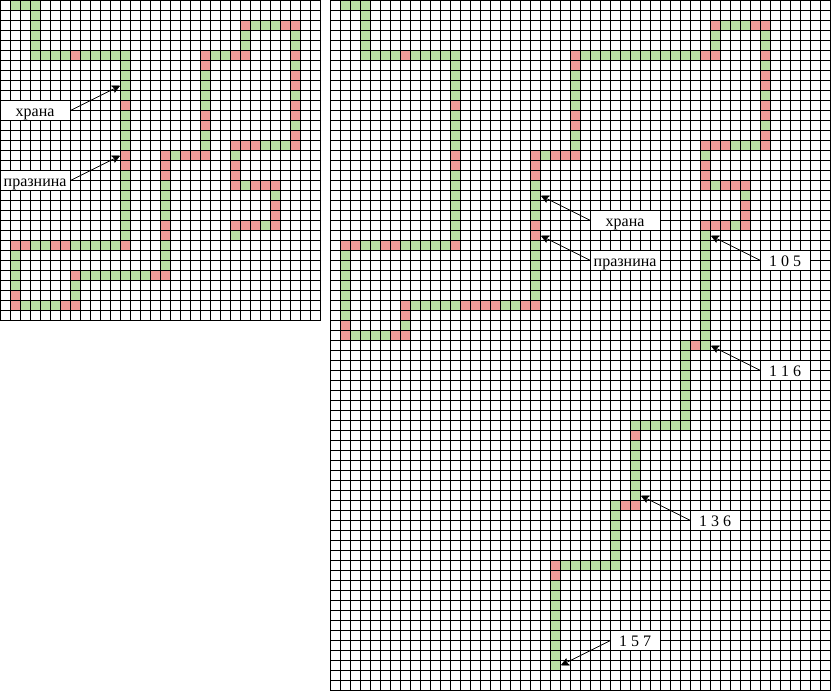
\includegraphics[scale=0.55]{santa_fe.png}
    \end{center}
    \caption{Изглед "Santa Fe" путање}
    \label{fig:santa_fe}
\end{figure}

Успешно је било проналажење све хране од стране робота у 21. генерацији за прву путању, а у 19. генерацији за другу путању. \cite{robo2} Овај проблем је решен уз помоћ програмског језика Lisp и коришћењем с-израза. \cite{lisp}
\subsection{Медицина}
Иако генетичко програмирање не може бити једино решење када се анализирају биолошки подаци, оно је важно као додатан аналитички алат који има потенцијал да пружи изненађујуће и непредвидиве резултате. Способност да пронађе корисне комбинације својстава и да их прикаже у облику разумљивом за људе га чине погодним за истраживање болести попут рака. \cite{cancer}

Коришћење унапређеног генетичког програмирања је показало боље резултате у проблему класификације података од класичних алгоритама машинског учења попут линеарне регресије, неуронских мрежа и класификације базиране на суседима. \cite{egp}
\subsection{Економија}
Можда једна од најбитнијих проблема са којима се сусреће ова дисциплина је предвиђање банкрупта компанија. Коришћењем генетичког програмирања дошло се до занимљивих карактеристика података ових предузећа. \cite{bankruptcy}

Такође, у економији је од велике важности предвидети податке на тржиштима хартија од вредности (берзама), како због смањења губитака од куповине и продаје акција, тако и зарад максимизовања профита. \cite{stock}

\section{Мета-генетичко програмирање}

Мета-генетичко програмирање подразумева упоредно еволуирање \textbf{(да ли је добар термин?)} програма који врши генетичко програмирање, које замењује ручно подешавање параметара и одлика алгоритма. 
\linebreak

\textbf{citat There is no reason to believe that having only one level of adaption in an evolutionary computation is optimal}. Обично су оператори генетичког програмирања унапред задати и фиксни, и најчешће се ради о комбинацији \textbf{propagation, crossover, mutation}, али су истраживани и неки алтернативни оператори \textbf{referenca?}, и испоставља се да у неким случајевима, коришћење тих алтернативних оператора, заједно са ,,класичним'' операторима даје боље резултате. Дакле, паметним одабиром и укључивањем одређених оператора мутације, могуће је постићи већи учинак програма који врши генетичко програмирање.
\linebreak

Међутим, одабир оператора није тривијалан, јер је могуће да неки јако добар оператор не буде ни лак за тумачење, ни интуитиван, односно, мало је вероватно да би нека особа сама осмислила такав оператор, што сасвим одговара мотивацији генетичких алгоритама уопште, где је простор претраге јако велик, и посао проналажења решења је препуштен рачунару, а не особи.
\linebreak

Као и у типичном генетичком програмирању, јединке \textbf{geni?} се приказују помоћу синтаксних стабала, с тим што оваква стабла садрже инструкције које представљају операторе мутације.
\linebreak

\textbf{fitness funkcija} узима у обзир могућност добијеног програма да ефикасно и ефективно еволуира програме, што укратко значи да је \textbf{fitness funkcija} самог програма који врши генетичко програмирање донекле сразмерна и \textbf{фитнес функцији} јединки које генерише.

\section{Osnovna uputstva}
Vaš seminarski rad mora da sadrži najmanje jednu \textbf{sliku}, najmanje jednu \textbf{tabelu} i najmanje \textbf{sedam referenci} u spisku literature. Najmanje jedna slika treba da bude originalna i da predstavlja neke podatke koje ste Vi osmislili da treba da prezentujete u svom radu. Isto važi i za najmanje jednu tabelu. 	Od referenci, neophodno je imati bar jednu \textbf{knjigu}, bar jedan \textbf{naučni članak} iz odgovarajućeg časopisa i bar jednu adekvatnu \textbf{veb adresu}. 

\textbf{Dužina seminarskog rada treba da bude od 10 do 12 strana.} Svako prekoračenje ili potkoračenje biće kažnjeno sa odgovarajućim brojem poena. Eventualno, nakon strane 12, može se javiti samo tekst poglavlja \textbf{Dodatak} koji sadrži nekakav dodatni k\^{o}d, ali je svakako potrebno da rad može da se pročita i razume i bez čitanja tog dodatka. 

Ко жели, може да пише рад ћирилицом. У том случају, неопходно је да су инсталирани одговарајући пакети: texlive-fonts-extra, texlive-latex-extra, texlive-lang-cyrillic, texlive-lang-other. 

Nemojte koristiti stari način pisanja slova, tj ovo:
\begin{verbatim}
\v{s} i \v{c} i \'c ...
\end{verbatim}
Koristite direknto naša slova:	
\begin{verbatim}
š i č i ć ... 
\end{verbatim}


\section{Engleski termini i citiranje}	
\label{sec:termini_i_citiranje}

Na svakom mestu u tekstu naglasiti odakle tačno potiču informacije. Uz sve novouvedene termine u zagradi naglasiti od koje engleske reči termin potiče. 

Naredni primeri ilustruju način uvođenja enlegskih termina kao i citiranje.

\begin{primer}
Problem zaustavljanja (eng.~{\em halting problem}) je neodlučiv \cite{haltingproblem}.
\end{primer}

\begin{primer}
Za prevođenje programa napisanih u programskom jeziku C može se koristiti GCC kompajler \cite{gcc}.
\end{primer}

\begin{primer}
 Da bi se ispitivala ispravost softvera, najpre je potrebno precizno definisati njegovo ponašanje \cite{laski2009software}. 
\end{primer}

Reference koje se koriste u ovom tekstu zadate su u datoteci {\em seminarski.bib}. Prevođenje u pdf format u Linux okruženju može se uraditi na sledeći način:
\begin{verbatim}
pdflatex TemaImePrezime.tex 
bibtex TemaImePrezime.aux 
pdflatex TemaImePrezime.tex 
pdflatex TemaImePrezime.tex 
\end{verbatim}
Prvo latexovanje je neophodno da bi se generisao {\em .aux} fajl. {\em bibtex} proizvodi odgovarajući {\em .bbl} fajl koji se koristi za generisanje literature. 
Potrebna su dva prolaza (dva puta pdflatex) da bi se reference ubacile u tekst (tj da ne bi ostali znakovi pitanja umesto referenci). Dodavanjem novih referenci potrebno je ponoviti ceo postupak.  











Broj naslova i podnaslova je proizvoljan. Neophodni su samo Uvod i Zaključak. Na poglavlja unutar teksta referisati se po potrebi. 
\begin{primer}
\end{primer}

Još jednom da napomenem da nema razloga da pišete:
\begin{verbatim}
\v{s} i \v{c} i \'c ...
\end{verbatim}
Možete koristiti srpska slova
\begin{verbatim}
š i č i ć ... 
\end{verbatim}



\section{Slike i tabele}
\label{slike_i_tabele}

Slike i tabele treba da budu u svom okruženju, sa odgovarajućim naslovima, obeležene labelom da koje omogućava referenciranje. 

\begin{primer} Ovako se ubacuje slika. Obratiti pažnju da je dodato i 
\begin{verbatim}
\usepackage{graphicx}
\end{verbatim}

\begin{figure}[h!]
\begin{center}
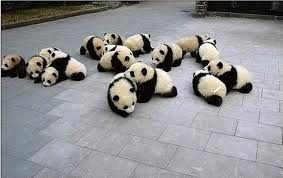
\includegraphics[scale=0.75]{panda.jpg}
\end{center}
\caption{Pande}
\label{fig:pande}
\end{figure}

Na svaku sliku neophodno je referisati se negde u tekstu. Na primer, na slici \ref{fig:pande} prikazane su pande. 
\end{primer}

\begin{primer} I tabele treba da budu u svom okruženju, i na njih je neophodno referisati se u tekstu. Na primer, u tabeli \ref{tab:tabela1} su prikazana različita poravnanja u tabelama.

\begin{table}[h!]
\begin{center}
\caption{Razlčita poravnanja u okviru iste tabele ne treba koristiti jer su nepregledna.}
\begin{tabular}{|c|l|r|} \hline
centralno poravnanje& levo poravnanje& desno poravnanje\\ \hline
a &b&c\\ \hline
d &e&f\\ \hline
\end{tabular}
\label{tab:tabela1}
\end{center}
\end{table}

\end{primer}

\section{K\^{o}d i paket listings}
Za ubacivanje koda koristite paket \textbf{listings}:
\url{https://en.wikibooks.org/wiki/LaTeX/Source_Code_Listings}

\begin{primer}
Primer ubacivanja koda za programski jezik Python dat je kroz listing \ref{simple}. Za neki drugi programski jezik, treba podesiti odgvarajući programski jezik u okviru defnisanja stila.
\end{primer}
\begin{lstlisting}[caption={Primer ubacivanja koda u tekst},frame=single, label=simple]
# This program adds up integers in the command line
import sys
try:
    total = sum(int(arg) for arg in sys.argv[1:])
    print 'sum =', total
except ValueError:
    print 'Please supply integer arguments'
\end{lstlisting}


\section{Закључак}
\label{sec:zakljucak}

Ovde pišem zaključak. 
Ovde pišem zaključak. 
Ovde pišem zaključak. 
Ovde pišem zaključak. 
Ovde pišem zaključak. 
Ovde pišem zaključak. 
Ovde pišem zaključak. 
Ovde pišem zaključak. 
Ovde pišem zaključak. 
Ovde pišem zaključak. 
Ovde pišem zaključak. 
Ovde pišem zaključak. 


\addcontentsline{toc}{section}{Literatura}
\appendix
\bibliography{literatura} 
\bibliographystyle{plain}

\appendix
\section{Dodatak}
Ovde pišem dodatne stvari, ukoliko za time ima potrebe.
Ovde pišem dodatne stvari, ukoliko za time ima potrebe.
Ovde pišem dodatne stvari, ukoliko za time ima potrebe.
Ovde pišem dodatne stvari, ukoliko za time ima potrebe.
Ovde pišem dodatne stvari, ukoliko za time ima potrebe.


\end{document}
